\documentclass[1p]{elsarticle_modified}
%\bibliographystyle{elsarticle-num}

%\usepackage[colorlinks]{hyperref}
%\usepackage{abbrmath_seonhwa} %\Abb, \Ascr, \Acal ,\Abf, \Afrak
\usepackage{amsfonts}
\usepackage{amssymb}
\usepackage{amsmath}
\usepackage{amsthm}
\usepackage{scalefnt}
\usepackage{amsbsy}
\usepackage{kotex}
\usepackage{caption}
\usepackage{subfig}
\usepackage{color}
\usepackage{graphicx}
\usepackage{xcolor} %% white, black, red, green, blue, cyan, magenta, yellow
\usepackage{float}
\usepackage{setspace}
\usepackage{hyperref}

\usepackage{tikz}
\usetikzlibrary{arrows}

\usepackage{multirow}
\usepackage{array} % fixed length table
\usepackage{hhline}

%%%%%%%%%%%%%%%%%%%%%
\makeatletter
\renewcommand*\env@matrix[1][\arraystretch]{%
	\edef\arraystretch{#1}%
	\hskip -\arraycolsep
	\let\@ifnextchar\new@ifnextchar
	\array{*\c@MaxMatrixCols c}}
\makeatother %https://tex.stackexchange.com/questions/14071/how-can-i-increase-the-line-spacing-in-a-matrix
%%%%%%%%%%%%%%%

\usepackage[normalem]{ulem}

\newcommand{\msout}[1]{\ifmmode\text{\sout{\ensuremath{#1}}}\else\sout{#1}\fi}
%SOURCE: \msout is \stkout macro in https://tex.stackexchange.com/questions/20609/strikeout-in-math-mode

\newcommand{\cancel}[1]{
	\ifmmode
	{\color{red}\msout{#1}}
	\else
	{\color{red}\sout{#1}}
	\fi
}

\newcommand{\add}[1]{
	{\color{blue}\uwave{#1}}
}

\newcommand{\replace}[2]{
	\ifmmode
	{\color{red}\msout{#1}}{\color{blue}\uwave{#2}}
	\else
	{\color{red}\sout{#1}}{\color{blue}\uwave{#2}}
	\fi
}

\newcommand{\Sol}{\mathcal{S}} %segment
\newcommand{\D}{D} %diagram
\newcommand{\A}{\mathcal{A}} %arc


%%%%%%%%%%%%%%%%%%%%%%%%%%%%%5 test

\def\sl{\operatorname{\textup{SL}}(2,\Cbb)}
\def\psl{\operatorname{\textup{PSL}}(2,\Cbb)}
\def\quan{\mkern 1mu \triangleright \mkern 1mu}

\theoremstyle{definition}
\newtheorem{thm}{Theorem}[section]
\newtheorem{prop}[thm]{Proposition}
\newtheorem{lem}[thm]{Lemma}
\newtheorem{ques}[thm]{Question}
\newtheorem{cor}[thm]{Corollary}
\newtheorem{defn}[thm]{Definition}
\newtheorem{exam}[thm]{Example}
\newtheorem{rmk}[thm]{Remark}
\newtheorem{alg}[thm]{Algorithm}

\newcommand{\I}{\sqrt{-1}}
\begin{document}

%\begin{frontmatter}
%
%\title{Boundary parabolic representations of knots up to 8 crossings}
%
%%% Group authors per affiliation:
%\author{Yunhi Cho} 
%\address{Department of Mathematics, University of Seoul, Seoul, Korea}
%\ead{yhcho@uos.ac.kr}
%
%
%\author{Seonhwa Kim} %\fnref{s_kim}}
%\address{Center for Geometry and Physics, Institute for Basic Science, Pohang, 37673, Korea}
%\ead{ryeona17@ibs.re.kr}
%
%\author{Hyuk Kim}
%\address{Department of Mathematical Sciences, Seoul National University, Seoul 08826, Korea}
%\ead{hyukkim@snu.ac.kr}
%
%\author{Seokbeom Yoon}
%\address{Department of Mathematical Sciences, Seoul National University, Seoul, 08826,  Korea}
%\ead{sbyoon15@snu.ac.kr}
%
%\begin{abstract}
%We find all boundary parabolic representation of knots up to 8 crossings.
%
%\end{abstract}
%\begin{keyword}
%    \MSC[2010] 57M25 
%\end{keyword}
%
%\end{frontmatter}

%\linenumbers
%\tableofcontents
%
\newcommand\colored[1]{\textcolor{white}{\rule[-0.35ex]{0.8em}{1.4ex}}\kern-0.8em\color{red} #1}%
%\newcommand\colored[1]{\textcolor{white}{ #1}\kern-2.17ex	\textcolor{white}{ #1}\kern-1.81ex	\textcolor{white}{ #1}\kern-2.15ex\color{red}#1	}

{\Large $\underline{12n_{0183}~(K12n_{0183})}$}

\setlength{\tabcolsep}{10pt}
\renewcommand{\arraystretch}{1.6}
\vspace{1cm}\begin{tabular}{m{100pt}>{\centering\arraybackslash}m{274pt}}
\multirow{5}{120pt}{
	\centering
	\includegraphics[width=112pt]{../../../GIT/diagram.site/Diagrams/png/2272_12n_0183.png}\\
\ \ \ A knot diagram\footnotemark}&
\allowdisplaybreaks
\textbf{Linearized knot diagam} \\
\cline{2-2}
 &
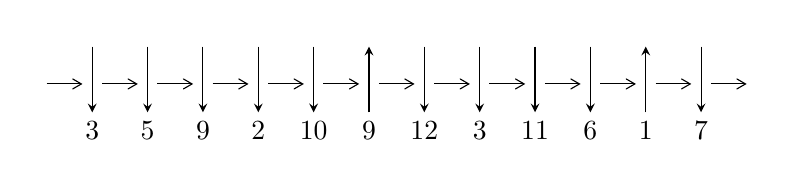
\begin{tikzpicture}[x=20pt, y=17pt]
	% nodes
	\node (C0) at (0, 0) {};
	\node (C1) at (1, 0) {};
	\node (C1U) at (1, +1) {};
	\node (C1D) at (1, -1) {3};

	\node (C2) at (2, 0) {};
	\node (C2U) at (2, +1) {};
	\node (C2D) at (2, -1) {5};

	\node (C3) at (3, 0) {};
	\node (C3U) at (3, +1) {};
	\node (C3D) at (3, -1) {9};

	\node (C4) at (4, 0) {};
	\node (C4U) at (4, +1) {};
	\node (C4D) at (4, -1) {2};

	\node (C5) at (5, 0) {};
	\node (C5U) at (5, +1) {};
	\node (C5D) at (5, -1) {10};

	\node (C6) at (6, 0) {};
	\node (C6U) at (6, +1) {};
	\node (C6D) at (6, -1) {9};

	\node (C7) at (7, 0) {};
	\node (C7U) at (7, +1) {};
	\node (C7D) at (7, -1) {12};

	\node (C8) at (8, 0) {};
	\node (C8U) at (8, +1) {};
	\node (C8D) at (8, -1) {3};

	\node (C9) at (9, 0) {};
	\node (C9U) at (9, +1) {};
	\node (C9D) at (9, -1) {11};

	\node (C10) at (10, 0) {};
	\node (C10U) at (10, +1) {};
	\node (C10D) at (10, -1) {6};

	\node (C11) at (11, 0) {};
	\node (C11U) at (11, +1) {};
	\node (C11D) at (11, -1) {1};

	\node (C12) at (12, 0) {};
	\node (C12U) at (12, +1) {};
	\node (C12D) at (12, -1) {7};
	\node (C13) at (13, 0) {};

	% arrows
	\draw[->,>={angle 60}]
	(C0) edge (C1) (C1) edge (C2) (C2) edge (C3) (C3) edge (C4) (C4) edge (C5) (C5) edge (C6) (C6) edge (C7) (C7) edge (C8) (C8) edge (C9) (C9) edge (C10) (C10) edge (C11) (C11) edge (C12) (C12) edge (C13) ;	\draw[->,>=stealth]
	(C1U) edge (C1D) (C2U) edge (C2D) (C3U) edge (C3D) (C4U) edge (C4D) (C5U) edge (C5D) (C6D) edge (C6U) (C7U) edge (C7D) (C8U) edge (C8D) (C9U) edge (C9D) (C10U) edge (C10D) (C11D) edge (C11U) (C12U) edge (C12D) ;
	\end{tikzpicture} \\
\hhline{~~} \\& 
\textbf{Solving Sequence} \\ \cline{2-2} 
 &
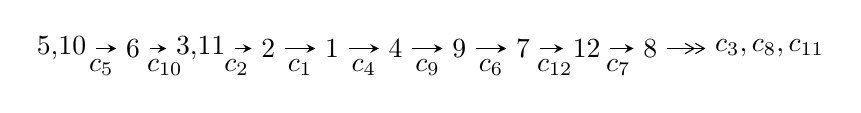
\begin{tikzpicture}[x=23pt, y=7pt]
	% node
	\node (A0) at (-1/8, 0) {5,10};
	\node (A1) at (1, 0) {6};
	\node (A2) at (33/16, 0) {3,11};
	\node (A3) at (25/8, 0) {2};
	\node (A4) at (33/8, 0) {1};
	\node (A5) at (41/8, 0) {4};
	\node (A6) at (49/8, 0) {9};
	\node (A7) at (57/8, 0) {7};
	\node (A8) at (65/8, 0) {12};
	\node (A9) at (73/8, 0) {8};
	\node (C1) at (1/2, -1) {$c_{5}$};
	\node (C2) at (3/2, -1) {$c_{10}$};
	\node (C3) at (21/8, -1) {$c_{2}$};
	\node (C4) at (29/8, -1) {$c_{1}$};
	\node (C5) at (37/8, -1) {$c_{4}$};
	\node (C6) at (45/8, -1) {$c_{9}$};
	\node (C7) at (53/8, -1) {$c_{6}$};
	\node (C8) at (61/8, -1) {$c_{12}$};
	\node (C9) at (69/8, -1) {$c_{7}$};
	\node (A10) at (11, 0) {$c_{3},c_{8},c_{11}$};

	% edge
	\draw[->,>=stealth]	
	(A0) edge (A1) (A1) edge (A2) (A2) edge (A3) (A3) edge (A4) (A4) edge (A5) (A5) edge (A6) (A6) edge (A7) (A7) edge (A8) (A8) edge (A9) ;
	\draw[->>,>={angle 60}]	
	(A9) edge (A10);
\end{tikzpicture} \\ 

\end{tabular} \\

\footnotetext{
The image of knot diagram is generated by the software ``\textbf{Draw programme}" developed by Andrew Bartholomew(\url{http://www.layer8.co.uk/maths/draw/index.htm\#Running-draw}), where we modified some parts for our purpose(\url{https://github.com/CATsTAILs/LinksPainter}).
}\phantom \\ \newline 
\centering \textbf{Ideals for irreducible components\footnotemark of $X_{\text{par}}$} 
 
\begin{align*}
I^u_{1}&=\langle 
-1.20523\times10^{32} u^{62}-1.33633\times10^{32} u^{61}+\cdots+4.02644\times10^{32} b+1.46507\times10^{32},\\
\phantom{I^u_{1}}&\phantom{= \langle  }1.44947\times10^{32} u^{62}-4.60820\times10^{30} u^{61}+\cdots+1.34215\times10^{32} a-2.19191\times10^{32},\;u^{63}+2 u^{62}+\cdots+4 u+1\rangle \\
I^u_{2}&=\langle 
b+1,\;2 u^8+u^7-5 u^6-3 u^5+4 u^4+3 u^3+2 u^2+a-2,\;u^9+u^8-2 u^7-3 u^6+u^5+3 u^4+2 u^3- u-1\rangle \\
\\
\end{align*}
\raggedright * 2 irreducible components of $\dim_{\mathbb{C}}=0$, with total 72 representations.\\
\footnotetext{All coefficients of polynomials are rational numbers. But the coefficients are sometimes approximated in decimal forms when there is not enough margin.}
\newpage
\renewcommand{\arraystretch}{1}
\centering \section*{I. $I^u_{1}= \langle -1.21\times10^{32} u^{62}-1.34\times10^{32} u^{61}+\cdots+4.03\times10^{32} b+1.47\times10^{32},\;1.45\times10^{32} u^{62}-4.61\times10^{30} u^{61}+\cdots+1.34\times10^{32} a-2.19\times10^{32},\;u^{63}+2 u^{62}+\cdots+4 u+1 \rangle$}
\flushleft \textbf{(i) Arc colorings}\\
\begin{tabular}{m{7pt} m{180pt} m{7pt} m{180pt} }
\flushright $a_{5}=$&$\begin{pmatrix}1\\0\end{pmatrix}$ \\
\flushright $a_{10}=$&$\begin{pmatrix}0\\u\end{pmatrix}$ \\
\flushright $a_{6}=$&$\begin{pmatrix}1\\u^2\end{pmatrix}$ \\
\flushright $a_{3}=$&$\begin{pmatrix}-1.07996 u^{62}+0.0343346 u^{61}+\cdots-1.91121 u+1.63313\\0.299329 u^{62}+0.331888 u^{61}+\cdots+1.56778 u-0.363863\end{pmatrix}$ \\
\flushright $a_{11}=$&$\begin{pmatrix}- u\\- u^3+u\end{pmatrix}$ \\
\flushright $a_{2}=$&$\begin{pmatrix}-0.780635 u^{62}+0.366222 u^{61}+\cdots-0.343427 u+1.26927\\0.299329 u^{62}+0.331888 u^{61}+\cdots+1.56778 u-0.363863\end{pmatrix}$ \\
\flushright $a_{1}=$&$\begin{pmatrix}0.498188 u^{62}+0.716504 u^{61}+\cdots+2.18592 u-0.0731899\\0.197906 u^{62}+0.176045 u^{61}+\cdots+1.05588 u+0.392848\end{pmatrix}$ \\
\flushright $a_{4}=$&$\begin{pmatrix}-1.09042 u^{62}-0.00217631 u^{61}+\cdots-1.99896 u+1.59173\\0.208603 u^{62}+0.265857 u^{61}+\cdots+1.12023 u-0.513655\end{pmatrix}$ \\
\flushright $a_{9}=$&$\begin{pmatrix}u^3\\u^5- u^3+u\end{pmatrix}$ \\
\flushright $a_{7}=$&$\begin{pmatrix}u^6- u^4+1\\u^8-2 u^6+2 u^4\end{pmatrix}$ \\
\flushright $a_{12}=$&$\begin{pmatrix}0.153458 u^{62}+0.0698033 u^{61}+\cdots+2.02811 u-0.0419731\\0.369503 u^{62}+0.349046 u^{61}+\cdots+2.10549 u+0.618121\end{pmatrix}$ \\
\flushright $a_{8}=$&$\begin{pmatrix}-0.445304 u^{62}-0.752007 u^{61}+\cdots-4.41211 u-0.301292\\0.301712 u^{62}+0.446342 u^{61}+\cdots+1.60552 u+0.343270\end{pmatrix}$\\&\end{tabular}
\flushleft \textbf{(ii) Obstruction class $= -1$}\\~\\
\flushleft \textbf{(iii) Cusp Shapes $= 20.7017 u^{62}+25.9299 u^{61}+\cdots+68.1832 u+9.80994$}\\~\\
\newpage\renewcommand{\arraystretch}{1}
\flushleft \textbf{(iv) u-Polynomials at the component}\newline \\
\begin{tabular}{m{50pt}|m{274pt}}
Crossings & \hspace{64pt}u-Polynomials at each crossing \\
\hline $$\begin{aligned}c_{1}\end{aligned}$$&$\begin{aligned}
&u^{63}+20 u^{62}+\cdots-54 u+1
\end{aligned}$\\
\hline $$\begin{aligned}c_{2},c_{4}\end{aligned}$$&$\begin{aligned}
&u^{63}-10 u^{62}+\cdots-6 u+1
\end{aligned}$\\
\hline $$\begin{aligned}c_{3},c_{8}\end{aligned}$$&$\begin{aligned}
&u^{63}+u^{62}+\cdots+5632 u+512
\end{aligned}$\\
\hline $$\begin{aligned}c_{5},c_{10}\end{aligned}$$&$\begin{aligned}
&u^{63}+2 u^{62}+\cdots+4 u+1
\end{aligned}$\\
\hline $$\begin{aligned}c_{6}\end{aligned}$$&$\begin{aligned}
&u^{63}+6 u^{62}+\cdots+1272 u+117
\end{aligned}$\\
\hline $$\begin{aligned}c_{7},c_{12}\end{aligned}$$&$\begin{aligned}
&u^{63}+2 u^{62}+\cdots+4 u+1
\end{aligned}$\\
\hline $$\begin{aligned}c_{9}\end{aligned}$$&$\begin{aligned}
&u^{63}+28 u^{62}+\cdots+6 u+1
\end{aligned}$\\
\hline $$\begin{aligned}c_{11}\end{aligned}$$&$\begin{aligned}
&u^{63}-36 u^{62}+\cdots+6 u+1
\end{aligned}$\\
\hline
\end{tabular}\\~\\
\newpage\renewcommand{\arraystretch}{1}
\flushleft \textbf{(v) Riley Polynomials at the component}\newline \\
\begin{tabular}{m{50pt}|m{274pt}}
Crossings & \hspace{64pt}Riley Polynomials at each crossing \\
\hline $$\begin{aligned}c_{1}\end{aligned}$$&$\begin{aligned}
&y^{63}+56 y^{62}+\cdots+398 y-1
\end{aligned}$\\
\hline $$\begin{aligned}c_{2},c_{4}\end{aligned}$$&$\begin{aligned}
&y^{63}-20 y^{62}+\cdots-54 y-1
\end{aligned}$\\
\hline $$\begin{aligned}c_{3},c_{8}\end{aligned}$$&$\begin{aligned}
&y^{63}+57 y^{62}+\cdots+10485760 y-262144
\end{aligned}$\\
\hline $$\begin{aligned}c_{5},c_{10}\end{aligned}$$&$\begin{aligned}
&y^{63}-28 y^{62}+\cdots+6 y-1
\end{aligned}$\\
\hline $$\begin{aligned}c_{6}\end{aligned}$$&$\begin{aligned}
&y^{63}-4 y^{62}+\cdots+236682 y-13689
\end{aligned}$\\
\hline $$\begin{aligned}c_{7},c_{12}\end{aligned}$$&$\begin{aligned}
&y^{63}+36 y^{62}+\cdots+6 y-1
\end{aligned}$\\
\hline $$\begin{aligned}c_{9}\end{aligned}$$&$\begin{aligned}
&y^{63}+16 y^{62}+\cdots-14 y-1
\end{aligned}$\\
\hline $$\begin{aligned}c_{11}\end{aligned}$$&$\begin{aligned}
&y^{63}-16 y^{62}+\cdots+90 y-1
\end{aligned}$\\
\hline
\end{tabular}\\~\\
\newpage\flushleft \textbf{(vi) Complex Volumes and Cusp Shapes}
$$\begin{array}{c|c|c}  
\text{Solutions to }I^u_{1}& \I (\text{vol} + \sqrt{-1}CS) & \text{Cusp shape}\\
 \hline 
\begin{aligned}
u &= \phantom{-}0.926110 + 0.366074 I \\
a &= -0.476922 + 0.252194 I \\
b &= -1.244610 + 0.271873 I\end{aligned}
 & -3.07412 - 1.36938 I & -14.1533 + 4.8337 I \\ \hline\begin{aligned}
u &= \phantom{-}0.926110 - 0.366074 I \\
a &= -0.476922 - 0.252194 I \\
b &= -1.244610 - 0.271873 I\end{aligned}
 & -3.07412 + 1.36938 I & -14.1533 - 4.8337 I \\ \hline\begin{aligned}
u &= -0.560970 + 0.838273 I \\
a &= -0.54543 + 1.39738 I \\
b &= \phantom{-}0.991983 - 0.885226 I\end{aligned}
 & \phantom{-}8.30126 + 6.53190 I & -3.98974 - 5.60044 I \\ \hline\begin{aligned}
u &= -0.560970 - 0.838273 I \\
a &= -0.54543 - 1.39738 I \\
b &= \phantom{-}0.991983 + 0.885226 I\end{aligned}
 & \phantom{-}8.30126 - 6.53190 I & -3.98974 + 5.60044 I \\ \hline\begin{aligned}
u &= \phantom{-}0.568620 + 0.802904 I \\
a &= -0.24496 - 1.43112 I \\
b &= \phantom{-}0.765553 + 0.905015 I\end{aligned}
 & \phantom{-}4.93754 - 1.39094 I & -6.19355 + 2.18855 I \\ \hline\begin{aligned}
u &= \phantom{-}0.568620 - 0.802904 I \\
a &= -0.24496 + 1.43112 I \\
b &= \phantom{-}0.765553 - 0.905015 I\end{aligned}
 & \phantom{-}4.93754 + 1.39094 I & -6.19355 - 2.18855 I \\ \hline\begin{aligned}
u &= -0.839102 + 0.489407 I \\
a &= \phantom{-}3.31553 + 9.53794 I \\
b &= -0.982885 + 0.004271 I\end{aligned}
 & \phantom{-}0.04887 + 2.03557 I & -112.9138 + 23.7044 I \\ \hline\begin{aligned}
u &= -0.839102 - 0.489407 I \\
a &= \phantom{-}3.31553 - 9.53794 I \\
b &= -0.982885 - 0.004271 I\end{aligned}
 & \phantom{-}0.04887 - 2.03557 I & -112.9138 - 23.7044 I \\ \hline\begin{aligned}
u &= -0.447997 + 0.861723 I \\
a &= -0.71326 - 1.29092 I \\
b &= \phantom{-}1.18245 + 0.86510 I\end{aligned}
 & \phantom{-}7.62161 - 10.39330 I & -4.76838 + 5.34490 I \\ \hline\begin{aligned}
u &= -0.447997 - 0.861723 I \\
a &= -0.71326 + 1.29092 I \\
b &= \phantom{-}1.18245 - 0.86510 I\end{aligned}
 & \phantom{-}7.62161 + 10.39330 I & -4.76838 - 5.34490 I\\
 \hline 
 \end{array}$$\newpage$$\begin{array}{c|c|c}  
\text{Solutions to }I^u_{1}& \I (\text{vol} + \sqrt{-1}CS) & \text{Cusp shape}\\
 \hline 
\begin{aligned}
u &= \phantom{-}0.772884 + 0.566946 I \\
a &= \phantom{-}0.741522 - 0.337818 I \\
b &= \phantom{-}0.0483031 + 0.1203760 I\end{aligned}
 & \phantom{-}1.79771 - 2.20109 I & -2.95390 + 4.60864 I \\ \hline\begin{aligned}
u &= \phantom{-}0.772884 - 0.566946 I \\
a &= \phantom{-}0.741522 + 0.337818 I \\
b &= \phantom{-}0.0483031 - 0.1203760 I\end{aligned}
 & \phantom{-}1.79771 + 2.20109 I & -2.95390 - 4.60864 I \\ \hline\begin{aligned}
u &= -0.529043 + 0.791579 I \\
a &= -0.17601 + 1.78351 I \\
b &= \phantom{-}0.710973 - 1.169850 I\end{aligned}
 & \phantom{-}9.18780 - 3.10441 I & -2.77684 + 1.28013 I \\ \hline\begin{aligned}
u &= -0.529043 - 0.791579 I \\
a &= -0.17601 - 1.78351 I \\
b &= \phantom{-}0.710973 + 1.169850 I\end{aligned}
 & \phantom{-}9.18780 + 3.10441 I & -2.77684 - 1.28013 I \\ \hline\begin{aligned}
u &= \phantom{-}0.427955 + 0.848872 I \\
a &= -0.482691 + 1.203200 I \\
b &= \phantom{-}1.039060 - 0.804035 I\end{aligned}
 & \phantom{-}4.08395 + 4.95084 I & -7.20670 - 2.70270 I \\ \hline\begin{aligned}
u &= \phantom{-}0.427955 - 0.848872 I \\
a &= -0.482691 - 1.203200 I \\
b &= \phantom{-}1.039060 + 0.804035 I\end{aligned}
 & \phantom{-}4.08395 - 4.95084 I & -7.20670 + 2.70270 I \\ \hline\begin{aligned}
u &= -0.916546 + 0.249573 I \\
a &= \phantom{-}0.527016 - 0.043315 I \\
b &= -1.008620 - 0.698143 I\end{aligned}
 & -1.65763 - 1.62708 I & -12.47188 + 3.53384 I \\ \hline\begin{aligned}
u &= -0.916546 - 0.249573 I \\
a &= \phantom{-}0.527016 + 0.043315 I \\
b &= -1.008620 + 0.698143 I\end{aligned}
 & -1.65763 + 1.62708 I & -12.47188 - 3.53384 I \\ \hline\begin{aligned}
u &= \phantom{-}0.972660 + 0.400781 I \\
a &= -0.570758 + 1.097760 I \\
b &= -1.45853 + 0.06110 I\end{aligned}
 & -3.33869 - 1.43594 I & -8.00000 + 0. I\phantom{ +0.000000I} \\ \hline\begin{aligned}
u &= \phantom{-}0.972660 - 0.400781 I \\
a &= -0.570758 - 1.097760 I \\
b &= -1.45853 - 0.06110 I\end{aligned}
 & -3.33869 + 1.43594 I & -8.00000 + 0. I\phantom{ +0.000000I}\\
 \hline 
 \end{array}$$\newpage$$\begin{array}{c|c|c}  
\text{Solutions to }I^u_{1}& \I (\text{vol} + \sqrt{-1}CS) & \text{Cusp shape}\\
 \hline 
\begin{aligned}
u &= -0.439813 + 0.813829 I \\
a &= -0.22505 - 1.43226 I \\
b &= \phantom{-}0.872307 + 0.941914 I\end{aligned}
 & \phantom{-}8.68256 - 0.17840 I & -3.11591 - 0.13366 I \\ \hline\begin{aligned}
u &= -0.439813 - 0.813829 I \\
a &= -0.22505 + 1.43226 I \\
b &= \phantom{-}0.872307 - 0.941914 I\end{aligned}
 & \phantom{-}8.68256 + 0.17840 I & -3.11591 + 0.13366 I \\ \hline\begin{aligned}
u &= \phantom{-}0.946126 + 0.549853 I \\
a &= \phantom{-}1.30038 + 1.55435 I \\
b &= -0.476073 - 0.045942 I\end{aligned}
 & \phantom{-}1.19543 - 2.08630 I & \phantom{-0.000000 } 0 \\ \hline\begin{aligned}
u &= \phantom{-}0.946126 - 0.549853 I \\
a &= \phantom{-}1.30038 - 1.55435 I \\
b &= -0.476073 + 0.045942 I\end{aligned}
 & \phantom{-}1.19543 + 2.08630 I & \phantom{-0.000000 } 0 \\ \hline\begin{aligned}
u &= -1.003650 + 0.458888 I \\
a &= -0.56877 - 1.84841 I \\
b &= -1.42816 + 0.42370 I\end{aligned}
 & -2.91315 + 4.52729 I & \phantom{-0.000000 } 0 \\ \hline\begin{aligned}
u &= -1.003650 - 0.458888 I \\
a &= -0.56877 + 1.84841 I \\
b &= -1.42816 - 0.42370 I\end{aligned}
 & -2.91315 - 4.52729 I & \phantom{-0.000000 } 0 \\ \hline\begin{aligned}
u &= \phantom{-}1.111750 + 0.078744 I \\
a &= \phantom{-}0.931682 - 0.009722 I \\
b &= \phantom{-}0.606356 - 0.865246 I\end{aligned}
 & \phantom{-}3.30246 - 1.91069 I & \phantom{-0.000000 } 0 \\ \hline\begin{aligned}
u &= \phantom{-}1.111750 - 0.078744 I \\
a &= \phantom{-}0.931682 + 0.009722 I \\
b &= \phantom{-}0.606356 + 0.865246 I\end{aligned}
 & \phantom{-}3.30246 + 1.91069 I & \phantom{-0.000000 } 0 \\ \hline\begin{aligned}
u &= -0.992246 + 0.519940 I \\
a &= -0.33704 - 1.95730 I \\
b &= -0.879799 + 0.608584 I\end{aligned}
 & -1.95839 + 4.15867 I & \phantom{-0.000000 } 0 \\ \hline\begin{aligned}
u &= -0.992246 - 0.519940 I \\
a &= -0.33704 + 1.95730 I \\
b &= -0.879799 - 0.608584 I\end{aligned}
 & -1.95839 - 4.15867 I & \phantom{-0.000000 } 0\\
 \hline 
 \end{array}$$\newpage$$\begin{array}{c|c|c}  
\text{Solutions to }I^u_{1}& \I (\text{vol} + \sqrt{-1}CS) & \text{Cusp shape}\\
 \hline 
\begin{aligned}
u &= \phantom{-}1.027300 + 0.547178 I \\
a &= -0.62187 + 1.64598 I \\
b &= -0.674886 - 1.080260 I\end{aligned}
 & \phantom{-}0.27233 - 7.55007 I & \phantom{-0.000000 } 0 \\ \hline\begin{aligned}
u &= \phantom{-}1.027300 - 0.547178 I \\
a &= -0.62187 - 1.64598 I \\
b &= -0.674886 + 1.080260 I\end{aligned}
 & \phantom{-}0.27233 + 7.55007 I & \phantom{-0.000000 } 0 \\ \hline\begin{aligned}
u &= \phantom{-}0.105288 + 0.803613 I \\
a &= \phantom{-}0.163733 + 0.190487 I \\
b &= \phantom{-}0.635693 - 0.133199 I\end{aligned}
 & -1.46958 + 2.74391 I & -2.52412 - 4.27240 I \\ \hline\begin{aligned}
u &= \phantom{-}0.105288 - 0.803613 I \\
a &= \phantom{-}0.163733 - 0.190487 I \\
b &= \phantom{-}0.635693 + 0.133199 I\end{aligned}
 & -1.46958 - 2.74391 I & -2.52412 + 4.27240 I \\ \hline\begin{aligned}
u &= -1.190260 + 0.105981 I \\
a &= \phantom{-}0.841204 + 0.034521 I \\
b &= \phantom{-}0.922740 + 0.637535 I\end{aligned}
 & -1.51798 - 2.46440 I & \phantom{-0.000000 } 0 \\ \hline\begin{aligned}
u &= -1.190260 - 0.105981 I \\
a &= \phantom{-}0.841204 - 0.034521 I \\
b &= \phantom{-}0.922740 - 0.637535 I\end{aligned}
 & -1.51798 + 2.46440 I & \phantom{-0.000000 } 0 \\ \hline\begin{aligned}
u &= \phantom{-}1.205040 + 0.067480 I \\
a &= \phantom{-}0.816284 + 0.015394 I \\
b &= \phantom{-}1.112880 - 0.749697 I\end{aligned}
 & \phantom{-}1.77097 + 7.99701 I & \phantom{-0.000000 } 0 \\ \hline\begin{aligned}
u &= \phantom{-}1.205040 - 0.067480 I \\
a &= \phantom{-}0.816284 - 0.015394 I \\
b &= \phantom{-}1.112880 + 0.749697 I\end{aligned}
 & \phantom{-}1.77097 - 7.99701 I & \phantom{-0.000000 } 0 \\ \hline\begin{aligned}
u &= \phantom{-}1.039570 + 0.658560 I \\
a &= -0.914741 + 0.261872 I \\
b &= \phantom{-}0.622398 - 0.949236 I\end{aligned}
 & \phantom{-}3.52241 - 4.08840 I & \phantom{-0.000000 } 0 \\ \hline\begin{aligned}
u &= \phantom{-}1.039570 - 0.658560 I \\
a &= -0.914741 - 0.261872 I \\
b &= \phantom{-}0.622398 + 0.949236 I\end{aligned}
 & \phantom{-}3.52241 + 4.08840 I & \phantom{-0.000000 } 0\\
 \hline 
 \end{array}$$\newpage$$\begin{array}{c|c|c}  
\text{Solutions to }I^u_{1}& \I (\text{vol} + \sqrt{-1}CS) & \text{Cusp shape}\\
 \hline 
\begin{aligned}
u &= -1.059960 + 0.641966 I \\
a &= -1.231410 - 0.420346 I \\
b &= \phantom{-}0.637529 + 1.260300 I\end{aligned}
 & \phantom{-}7.59858 + 8.49760 I & \phantom{-0.000000 } 0 \\ \hline\begin{aligned}
u &= -1.059960 - 0.641966 I \\
a &= -1.231410 + 0.420346 I \\
b &= \phantom{-}0.637529 - 1.260300 I\end{aligned}
 & \phantom{-}7.59858 - 8.49760 I & \phantom{-0.000000 } 0 \\ \hline\begin{aligned}
u &= -1.057440 + 0.680554 I \\
a &= -1.002810 + 0.058966 I \\
b &= \phantom{-}0.898990 + 0.875767 I\end{aligned}
 & \phantom{-}6.80806 - 0.88135 I & \phantom{-0.000000 } 0 \\ \hline\begin{aligned}
u &= -1.057440 - 0.680554 I \\
a &= -1.002810 - 0.058966 I \\
b &= \phantom{-}0.898990 - 0.875767 I\end{aligned}
 & \phantom{-}6.80806 + 0.88135 I & \phantom{-0.000000 } 0 \\ \hline\begin{aligned}
u &= \phantom{-}0.568628 + 0.459189 I \\
a &= \phantom{-}1.57734 + 0.31772 I \\
b &= -0.253084 - 0.388928 I\end{aligned}
 & \phantom{-}2.13125 - 2.17129 I & -3.22626 + 3.56149 I \\ \hline\begin{aligned}
u &= \phantom{-}0.568628 - 0.459189 I \\
a &= \phantom{-}1.57734 - 0.31772 I \\
b &= -0.253084 + 0.388928 I\end{aligned}
 & \phantom{-}2.13125 + 2.17129 I & -3.22626 - 3.56149 I \\ \hline\begin{aligned}
u &= -1.206380 + 0.395280 I \\
a &= \phantom{-}0.870666 + 0.422612 I \\
b &= \phantom{-}0.706799 - 0.004491 I\end{aligned}
 & -5.38670 + 1.34424 I & \phantom{-0.000000 } 0 \\ \hline\begin{aligned}
u &= -1.206380 - 0.395280 I \\
a &= \phantom{-}0.870666 - 0.422612 I \\
b &= \phantom{-}0.706799 + 0.004491 I\end{aligned}
 & -5.38670 - 1.34424 I & \phantom{-0.000000 } 0 \\ \hline\begin{aligned}
u &= -1.109200 + 0.619508 I \\
a &= \phantom{-}1.24867 + 1.72679 I \\
b &= \phantom{-}0.939930 - 0.857494 I\end{aligned}
 & \phantom{-}6.67687 + 5.54473 I & \phantom{-0.000000 } 0 \\ \hline\begin{aligned}
u &= -1.109200 - 0.619508 I \\
a &= \phantom{-}1.24867 - 1.72679 I \\
b &= \phantom{-}0.939930 + 0.857494 I\end{aligned}
 & \phantom{-}6.67687 - 5.54473 I & \phantom{-0.000000 } 0\\
 \hline 
 \end{array}$$\newpage$$\begin{array}{c|c|c}  
\text{Solutions to }I^u_{1}& \I (\text{vol} + \sqrt{-1}CS) & \text{Cusp shape}\\
 \hline 
\begin{aligned}
u &= \phantom{-}0.452256 + 0.561618 I \\
a &= \phantom{-}1.40155 - 1.36845 I \\
b &= -0.506448 + 0.882679 I\end{aligned}
 & \phantom{-}1.87503 + 3.06479 I & -4.36652 - 4.78234 I \\ \hline\begin{aligned}
u &= \phantom{-}0.452256 - 0.561618 I \\
a &= \phantom{-}1.40155 + 1.36845 I \\
b &= -0.506448 - 0.882679 I\end{aligned}
 & \phantom{-}1.87503 - 3.06479 I & -4.36652 + 4.78234 I \\ \hline\begin{aligned}
u &= \phantom{-}1.124570 + 0.631526 I \\
a &= \phantom{-}0.93240 - 1.80350 I \\
b &= \phantom{-}1.123120 + 0.773338 I\end{aligned}
 & \phantom{-}1.99016 - 10.45010 I & \phantom{-0.000000 } 0 \\ \hline\begin{aligned}
u &= \phantom{-}1.124570 - 0.631526 I \\
a &= \phantom{-}0.93240 + 1.80350 I \\
b &= \phantom{-}1.123120 - 0.773338 I\end{aligned}
 & \phantom{-}1.99016 + 10.45010 I & \phantom{-0.000000 } 0 \\ \hline\begin{aligned}
u &= -1.120990 + 0.642900 I \\
a &= \phantom{-}0.86354 + 2.02077 I \\
b &= \phantom{-}1.24190 - 0.85165 I\end{aligned}
 & \phantom{-}5.5911 + 15.9697 I & \phantom{-0.000000 } 0 \\ \hline\begin{aligned}
u &= -1.120990 - 0.642900 I \\
a &= \phantom{-}0.86354 - 2.02077 I \\
b &= \phantom{-}1.24190 + 0.85165 I\end{aligned}
 & \phantom{-}5.5911 - 15.9697 I & \phantom{-0.000000 } 0 \\ \hline\begin{aligned}
u &= \phantom{-}1.198640 + 0.490741 I \\
a &= \phantom{-}0.872834 - 0.659332 I \\
b &= \phantom{-}0.755641 + 0.177473 I\end{aligned}
 & -4.71317 - 7.47420 I & \phantom{-0.000000 } 0 \\ \hline\begin{aligned}
u &= \phantom{-}1.198640 - 0.490741 I \\
a &= \phantom{-}0.872834 + 0.659332 I \\
b &= \phantom{-}0.755641 - 0.177473 I\end{aligned}
 & -4.71317 + 7.47420 I & \phantom{-0.000000 } 0 \\ \hline\begin{aligned}
u &= -0.575685 + 0.399556 I \\
a &= \phantom{-}1.31366 + 0.78416 I \\
b &= -0.548676 - 0.386355 I\end{aligned}
 & -0.700698 - 0.064745 I & -10.52169 + 0.11838 I \\ \hline\begin{aligned}
u &= -0.575685 - 0.399556 I \\
a &= \phantom{-}1.31366 - 0.78416 I \\
b &= -0.548676 + 0.386355 I\end{aligned}
 & -0.700698 + 0.064745 I & -10.52169 - 0.11838 I\\
 \hline 
 \end{array}$$\newpage$$\begin{array}{c|c|c}  
\text{Solutions to }I^u_{1}& \I (\text{vol} + \sqrt{-1}CS) & \text{Cusp shape}\\
 \hline 
\begin{aligned}
u &= -0.505150\phantom{ +0.000000I} \\
a &= \phantom{-}1.23248\phantom{ +0.000000I} \\
b &= -0.339414\phantom{ +0.000000I}\end{aligned}
 & -0.801265\phantom{ +0.000000I} & -12.3320\phantom{ +0.000000I} \\ \hline\begin{aligned}
u &= -0.145540 + 0.342331 I \\
a &= \phantom{-}2.27747 + 0.36324 I \\
b &= -1.183120 - 0.244413 I\end{aligned}
 & -1.04760 - 1.10754 I & -6.89009 + 0.60196 I \\ \hline\begin{aligned}
u &= -0.145540 - 0.342331 I \\
a &= \phantom{-}2.27747 - 0.36324 I \\
b &= -1.183120 + 0.244413 I\end{aligned}
 & -1.04760 + 1.10754 I & -6.89009 - 0.60196 I\\
 \hline 
 \end{array}$$\newpage\newpage\renewcommand{\arraystretch}{1}
\centering \section*{II. $I^u_{2}= \langle b+1,\;2 u^8+u^7+\cdots+a-2,\;u^9+u^8-2 u^7-3 u^6+u^5+3 u^4+2 u^3- u-1 \rangle$}
\flushleft \textbf{(i) Arc colorings}\\
\begin{tabular}{m{7pt} m{180pt} m{7pt} m{180pt} }
\flushright $a_{5}=$&$\begin{pmatrix}1\\0\end{pmatrix}$ \\
\flushright $a_{10}=$&$\begin{pmatrix}0\\u\end{pmatrix}$ \\
\flushright $a_{6}=$&$\begin{pmatrix}1\\u^2\end{pmatrix}$ \\
\flushright $a_{3}=$&$\begin{pmatrix}-2 u^8- u^7+5 u^6+3 u^5-4 u^4-3 u^3-2 u^2+2\\-1\end{pmatrix}$ \\
\flushright $a_{11}=$&$\begin{pmatrix}- u\\- u^3+u\end{pmatrix}$ \\
\flushright $a_{2}=$&$\begin{pmatrix}-2 u^8- u^7+5 u^6+3 u^5-4 u^4-3 u^3-2 u^2+1\\-1\end{pmatrix}$ \\
\flushright $a_{1}=$&$\begin{pmatrix}-1\\0\end{pmatrix}$ \\
\flushright $a_{4}=$&$\begin{pmatrix}-2 u^8- u^7+5 u^6+3 u^5-4 u^4-3 u^3-2 u^2+2\\-1\end{pmatrix}$ \\
\flushright $a_{9}=$&$\begin{pmatrix}u^3\\u^5- u^3+u\end{pmatrix}$ \\
\flushright $a_{7}=$&$\begin{pmatrix}u^6- u^4+1\\u^8-2 u^6+2 u^4\end{pmatrix}$ \\
\flushright $a_{12}=$&$\begin{pmatrix}- u^3\\- u^3+u\end{pmatrix}$ \\
\flushright $a_{8}=$&$\begin{pmatrix}u^3\\u^5- u^3+u\end{pmatrix}$\\&\end{tabular}
\flushleft \textbf{(ii) Obstruction class $= 1$}\\~\\
\flushleft \textbf{(iii) Cusp Shapes $= 6 u^8-5 u^7-10 u^6+8 u^5+10 u^4-8 u^3+4 u^2-8 u-10$}\\~\\
\newpage\renewcommand{\arraystretch}{1}
\flushleft \textbf{(iv) u-Polynomials at the component}\newline \\
\begin{tabular}{m{50pt}|m{274pt}}
Crossings & \hspace{64pt}u-Polynomials at each crossing \\
\hline $$\begin{aligned}c_{1},c_{2}\end{aligned}$$&$\begin{aligned}
&(u-1)^9
\end{aligned}$\\
\hline $$\begin{aligned}c_{3},c_{8}\end{aligned}$$&$\begin{aligned}
&u^9
\end{aligned}$\\
\hline $$\begin{aligned}c_{4}\end{aligned}$$&$\begin{aligned}
&(u+1)^9
\end{aligned}$\\
\hline $$\begin{aligned}c_{5}\end{aligned}$$&$\begin{aligned}
&u^9+u^8-2 u^7-3 u^6+u^5+3 u^4+2 u^3- u-1
\end{aligned}$\\
\hline $$\begin{aligned}c_{6},c_{11}\end{aligned}$$&$\begin{aligned}
&u^9+3 u^8+8 u^7+13 u^6+17 u^5+17 u^4+12 u^3+6 u^2+u-1
\end{aligned}$\\
\hline $$\begin{aligned}c_{7}\end{aligned}$$&$\begin{aligned}
&u^9+u^8+2 u^7+u^6+3 u^5+u^4+2 u^3+u-1
\end{aligned}$\\
\hline $$\begin{aligned}c_{9}\end{aligned}$$&$\begin{aligned}
&u^9-5 u^8+12 u^7-15 u^6+9 u^5+u^4-4 u^3+2 u^2+u-1
\end{aligned}$\\
\hline $$\begin{aligned}c_{10}\end{aligned}$$&$\begin{aligned}
&u^9- u^8-2 u^7+3 u^6+u^5-3 u^4+2 u^3- u+1
\end{aligned}$\\
\hline $$\begin{aligned}c_{12}\end{aligned}$$&$\begin{aligned}
&u^9- u^8+2 u^7- u^6+3 u^5- u^4+2 u^3+u+1
\end{aligned}$\\
\hline
\end{tabular}\\~\\
\newpage\renewcommand{\arraystretch}{1}
\flushleft \textbf{(v) Riley Polynomials at the component}\newline \\
\begin{tabular}{m{50pt}|m{274pt}}
Crossings & \hspace{64pt}Riley Polynomials at each crossing \\
\hline $$\begin{aligned}c_{1},c_{2},c_{4}\end{aligned}$$&$\begin{aligned}
&(y-1)^9
\end{aligned}$\\
\hline $$\begin{aligned}c_{3},c_{8}\end{aligned}$$&$\begin{aligned}
&y^9
\end{aligned}$\\
\hline $$\begin{aligned}c_{5},c_{10}\end{aligned}$$&$\begin{aligned}
&y^9-5 y^8+12 y^7-15 y^6+9 y^5+y^4-4 y^3+2 y^2+y-1
\end{aligned}$\\
\hline $$\begin{aligned}c_{6},c_{11}\end{aligned}$$&$\begin{aligned}
&y^9+7 y^8+20 y^7+25 y^6+5 y^5-15 y^4+22 y^2+13 y-1
\end{aligned}$\\
\hline $$\begin{aligned}c_{7},c_{12}\end{aligned}$$&$\begin{aligned}
&y^9+3 y^8+8 y^7+13 y^6+17 y^5+17 y^4+12 y^3+6 y^2+y-1
\end{aligned}$\\
\hline $$\begin{aligned}c_{9}\end{aligned}$$&$\begin{aligned}
&y^9- y^8+12 y^7-7 y^6+37 y^5+y^4-10 y^2+5 y-1
\end{aligned}$\\
\hline
\end{tabular}\\~\\
\newpage\flushleft \textbf{(vi) Complex Volumes and Cusp Shapes}
$$\begin{array}{c|c|c}  
\text{Solutions to }I^u_{2}& \I (\text{vol} + \sqrt{-1}CS) & \text{Cusp shape}\\
 \hline 
\begin{aligned}
u &= -0.772920 + 0.510351 I \\
a &= \phantom{-}1.67861 + 2.31573 I \\
b &= -1.00000\phantom{ +0.000000I}\end{aligned}
 & \phantom{-}0.13850 + 2.09337 I & \phantom{-}0.6725 - 14.2088 I \\ \hline\begin{aligned}
u &= -0.772920 - 0.510351 I \\
a &= \phantom{-}1.67861 - 2.31573 I \\
b &= -1.00000\phantom{ +0.000000I}\end{aligned}
 & \phantom{-}0.13850 - 2.09337 I & \phantom{-}0.6725 + 14.2088 I \\ \hline\begin{aligned}
u &= \phantom{-}0.825933\phantom{ +0.000000I} \\
a &= -0.871015\phantom{ +0.000000I} \\
b &= -1.00000\phantom{ +0.000000I}\end{aligned}
 & -2.84338\phantom{ +0.000000I} & -13.8440\phantom{ +0.000000I} \\ \hline\begin{aligned}
u &= \phantom{-}1.173910 + 0.391555 I \\
a &= -0.893484 + 0.630694 I \\
b &= -1.00000\phantom{ +0.000000I}\end{aligned}
 & -6.01628 - 1.33617 I & -18.6190 + 0.6500 I \\ \hline\begin{aligned}
u &= \phantom{-}1.173910 - 0.391555 I \\
a &= -0.893484 - 0.630694 I \\
b &= -1.00000\phantom{ +0.000000I}\end{aligned}
 & -6.01628 + 1.33617 I & -18.6190 - 0.6500 I \\ \hline\begin{aligned}
u &= -0.141484 + 0.739668 I \\
a &= \phantom{-}0.309843 + 0.043204 I \\
b &= -1.00000\phantom{ +0.000000I}\end{aligned}
 & -2.26187 - 2.45442 I & -11.89962 + 1.90984 I \\ \hline\begin{aligned}
u &= -0.141484 - 0.739668 I \\
a &= \phantom{-}0.309843 - 0.043204 I \\
b &= -1.00000\phantom{ +0.000000I}\end{aligned}
 & -2.26187 + 2.45442 I & -11.89962 - 1.90984 I \\ \hline\begin{aligned}
u &= -1.172470 + 0.500383 I \\
a &= -0.659464 - 0.874093 I \\
b &= -1.00000\phantom{ +0.000000I}\end{aligned}
 & -5.24306 + 7.08493 I & -15.2318 - 2.9321 I \\ \hline\begin{aligned}
u &= -1.172470 - 0.500383 I \\
a &= -0.659464 + 0.874093 I \\
b &= -1.00000\phantom{ +0.000000I}\end{aligned}
 & -5.24306 - 7.08493 I & -15.2318 + 2.9321 I\\
 \hline 
 \end{array}$$\newpage
\newpage\renewcommand{\arraystretch}{1}
\centering \section*{ III. u-Polynomials}
\begin{tabular}{m{50pt}|m{274pt}}
Crossings & \hspace{64pt}u-Polynomials at each crossing \\
\hline $$\begin{aligned}c_{1}\end{aligned}$$&$\begin{aligned}
&((u-1)^9)(u^{63}+20 u^{62}+\cdots-54 u+1)
\end{aligned}$\\
\hline $$\begin{aligned}c_{2}\end{aligned}$$&$\begin{aligned}
&((u-1)^9)(u^{63}-10 u^{62}+\cdots-6 u+1)
\end{aligned}$\\
\hline $$\begin{aligned}c_{3},c_{8}\end{aligned}$$&$\begin{aligned}
&u^9(u^{63}+u^{62}+\cdots+5632 u+512)
\end{aligned}$\\
\hline $$\begin{aligned}c_{4}\end{aligned}$$&$\begin{aligned}
&((u+1)^9)(u^{63}-10 u^{62}+\cdots-6 u+1)
\end{aligned}$\\
\hline $$\begin{aligned}c_{5}\end{aligned}$$&$\begin{aligned}
&(u^9+u^8+\cdots- u-1)(u^{63}+2 u^{62}+\cdots+4 u+1)
\end{aligned}$\\
\hline $$\begin{aligned}c_{6}\end{aligned}$$&$\begin{aligned}
&(u^9+3 u^8+8 u^7+13 u^6+17 u^5+17 u^4+12 u^3+6 u^2+u-1)\\
&\cdot(u^{63}+6 u^{62}+\cdots+1272 u+117)
\end{aligned}$\\
\hline $$\begin{aligned}c_{7}\end{aligned}$$&$\begin{aligned}
&(u^9+u^8+\cdots+u-1)(u^{63}+2 u^{62}+\cdots+4 u+1)
\end{aligned}$\\
\hline $$\begin{aligned}c_{9}\end{aligned}$$&$\begin{aligned}
&(u^9-5 u^8+12 u^7-15 u^6+9 u^5+u^4-4 u^3+2 u^2+u-1)\\
&\cdot(u^{63}+28 u^{62}+\cdots+6 u+1)
\end{aligned}$\\
\hline $$\begin{aligned}c_{10}\end{aligned}$$&$\begin{aligned}
&(u^9- u^8+\cdots- u+1)(u^{63}+2 u^{62}+\cdots+4 u+1)
\end{aligned}$\\
\hline $$\begin{aligned}c_{11}\end{aligned}$$&$\begin{aligned}
&(u^9+3 u^8+8 u^7+13 u^6+17 u^5+17 u^4+12 u^3+6 u^2+u-1)\\
&\cdot(u^{63}-36 u^{62}+\cdots+6 u+1)
\end{aligned}$\\
\hline $$\begin{aligned}c_{12}\end{aligned}$$&$\begin{aligned}
&(u^9- u^8+\cdots+u+1)(u^{63}+2 u^{62}+\cdots+4 u+1)
\end{aligned}$\\
\hline
\end{tabular}\newpage\renewcommand{\arraystretch}{1}
\centering \section*{ IV. Riley Polynomials}
\begin{tabular}{m{50pt}|m{274pt}}
Crossings & \hspace{64pt}Riley Polynomials at each crossing \\
\hline $$\begin{aligned}c_{1}\end{aligned}$$&$\begin{aligned}
&((y-1)^9)(y^{63}+56 y^{62}+\cdots+398 y-1)
\end{aligned}$\\
\hline $$\begin{aligned}c_{2},c_{4}\end{aligned}$$&$\begin{aligned}
&((y-1)^9)(y^{63}-20 y^{62}+\cdots-54 y-1)
\end{aligned}$\\
\hline $$\begin{aligned}c_{3},c_{8}\end{aligned}$$&$\begin{aligned}
&y^9(y^{63}+57 y^{62}+\cdots+1.04858\times10^{7} y-262144)
\end{aligned}$\\
\hline $$\begin{aligned}c_{5},c_{10}\end{aligned}$$&$\begin{aligned}
&(y^9-5 y^8+12 y^7-15 y^6+9 y^5+y^4-4 y^3+2 y^2+y-1)\\
&\cdot(y^{63}-28 y^{62}+\cdots+6 y-1)
\end{aligned}$\\
\hline $$\begin{aligned}c_{6}\end{aligned}$$&$\begin{aligned}
&(y^9+7 y^8+20 y^7+25 y^6+5 y^5-15 y^4+22 y^2+13 y-1)\\
&\cdot(y^{63}-4 y^{62}+\cdots+236682 y-13689)
\end{aligned}$\\
\hline $$\begin{aligned}c_{7},c_{12}\end{aligned}$$&$\begin{aligned}
&(y^9+3 y^8+8 y^7+13 y^6+17 y^5+17 y^4+12 y^3+6 y^2+y-1)\\
&\cdot(y^{63}+36 y^{62}+\cdots+6 y-1)
\end{aligned}$\\
\hline $$\begin{aligned}c_{9}\end{aligned}$$&$\begin{aligned}
&(y^9- y^8+12 y^7-7 y^6+37 y^5+y^4-10 y^2+5 y-1)\\
&\cdot(y^{63}+16 y^{62}+\cdots-14 y-1)
\end{aligned}$\\
\hline $$\begin{aligned}c_{11}\end{aligned}$$&$\begin{aligned}
&(y^9+7 y^8+20 y^7+25 y^6+5 y^5-15 y^4+22 y^2+13 y-1)\\
&\cdot(y^{63}-16 y^{62}+\cdots+90 y-1)
\end{aligned}$\\
\hline
\end{tabular}
\vskip 2pc
\end{document}